\chapter{Introduction\label{cha:chapter1}}

The number of interconnected devices on the Internet is constantly increasing, more and more data is exchanged between different participants.
While the Internet initially experienced a broad distribution during the 80s thanks to the world wide web service, where mainly personal computers and enterprise servers were involved in the communication, nowadays the number of offered services and online devices is countless.
Over the last few years, \textit{Internet of Things (IoT)} has become very popular and an end to this trend is not predictable.
All kinds of different devices are connected to the Internet (e.g. smartphones, smart watches, smart TVs, smart home devices, cars) and exchanging data with each other.
Thus, the amount of exchanged data over the Internet and between network nodes is constantly increasing as well, leading to higher requirements on the overall network infrastructure to ensure a high connection quality with little delays as well as to avoid network congestion.\\

A common scenario is devices communicating with each other via a cloud server in a big data center, where the physical distance between devices might be relatively far.
Often though, and this is especially the case for IoT scenarios, a lot of data is produced and consumed locally, on the edge of networks.
While this is not a big deal for services which don’t have a high real-time requirement, a service that has a high real-time requirement relies on the network connection quality and low delay times between participating devices.
If this cannot be ensured, the service is unusable.
This becomes even more important in applications where personal safety plays a role.
For example, when a device at the side of the road communicates with an autonomous car and instructs to brake.
If these devices were interconnected via a server in the cloud, the delay time would depend on the current network congestion level, resulting in a varying time in delay, thus not ensuring the \textit{quality of service (QoS)}.
This issue is addressed by Fog computing.\\

\textit{Fog computing} provides a distributed infrastructure at the edge of the network, resulting in low-latency access and faster response to application requests \cite{mobility-aware-scheduling}.
In a fog infrastructure, there is a variable number of so called fog nodes, which can provide resources like computation or storage.
Fog nodes are usually small devices with limited resources compared to servers in the cloud.
Furthermore, fog nodes in a fog infrastructure are not necessarily of the same kind, thus they have a different amount of resources available.
For example, one fog node can have a relatively low computation power compared to another fog node.
The challenge here is to distribute the services among different fog nodes while ensuring the QoS requirements are met.
While some services can’t be executed at all on certain nodes due to the lack of resources, other services are competing for resources on other fog nodes.
One solution here is to \textit{decompose} services into smaller \textit{tasks}, so that these tasks could run on different fog nodes.
However, these tasks need to be recomposed thereafter to provide the service as a whole.
This part is called \textit{service composition} and is illustrated in figure \ref{fig:service-composition}.\\

\begin{figure}
    \centering
    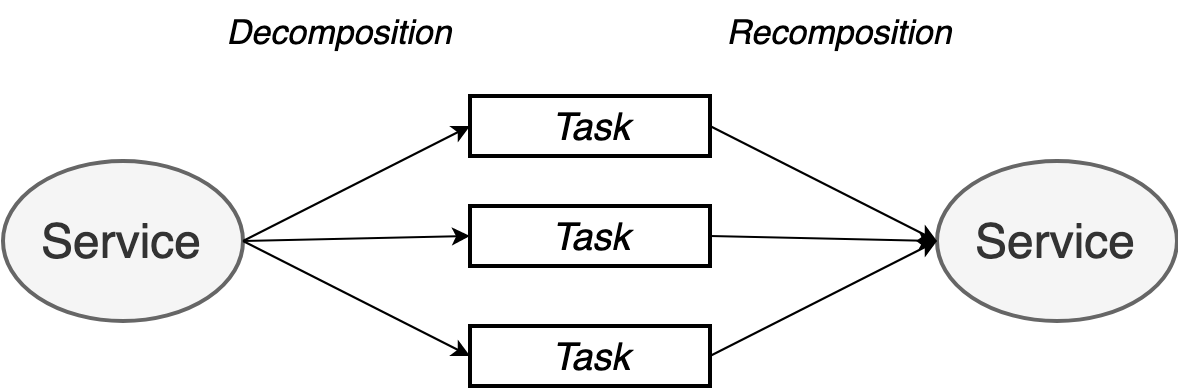
\includegraphics[width=12cm]{service-composition}
    \caption{Service Composition}
    \label{fig:service-composition}
\end{figure}

The challenge here is though, that the conditions inside of the fog infrastructure can change at any time.
First of all, the demand for the offered services can increase or decrease at any point in time.
Furthermore, fog nodes can join or leave the network at any point in time.
Simply put, tasks have to be distributed \textit{dynamically}.
To ensure that every service meets the QoS requirements, every node has to be constantly monitored.
If the demand for services increases, the average load on the fog nodes will be high.
To still provide an acceptable service quality for each service, tasks of services which have lower QoS requirements have to be moved to another resource.
A task could always be executed in the cloud, but this would lead to longer delay times.